%Task 6
\input{baseHoja.tex}
\begin{document}

\section*{Task 6}
In this section, a D Flip-Flop and a SR Latch
are implemented, based on logic gates.
\subsection*{SR Latch}
For the SR Latch, it is 
implemented using NOR gates of 74HC02 integrated
circuit. The resulting schematic is shown below.

\begin{figure}[H]
    \begin{centering}
    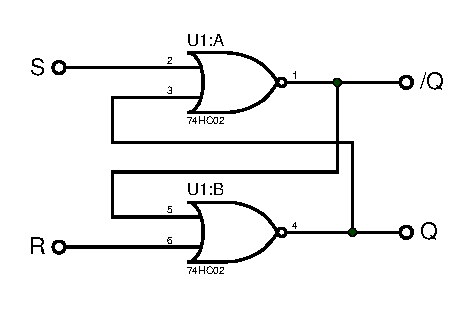
\includegraphics[width=0.4\textwidth]{latchSR}
    \par\end{centering}
    \caption{SR Latch circuit - Made in Proteus 7.8}
\end{figure}

PARAMETROS IMPORTANTES: PROPAGACION DE SET O 
RESET A LAS SALIDAS. MEDIR. COMPARAR CON UNO
COMERCIAL CUALQUIERA

\subsection*{D Flip-Flop}
For the D flip-flop, it is implemented using 
the SR Latch designed before, adding the 
remaining parts as shown below.

\begin{figure}[H]
    \begin{centering}
    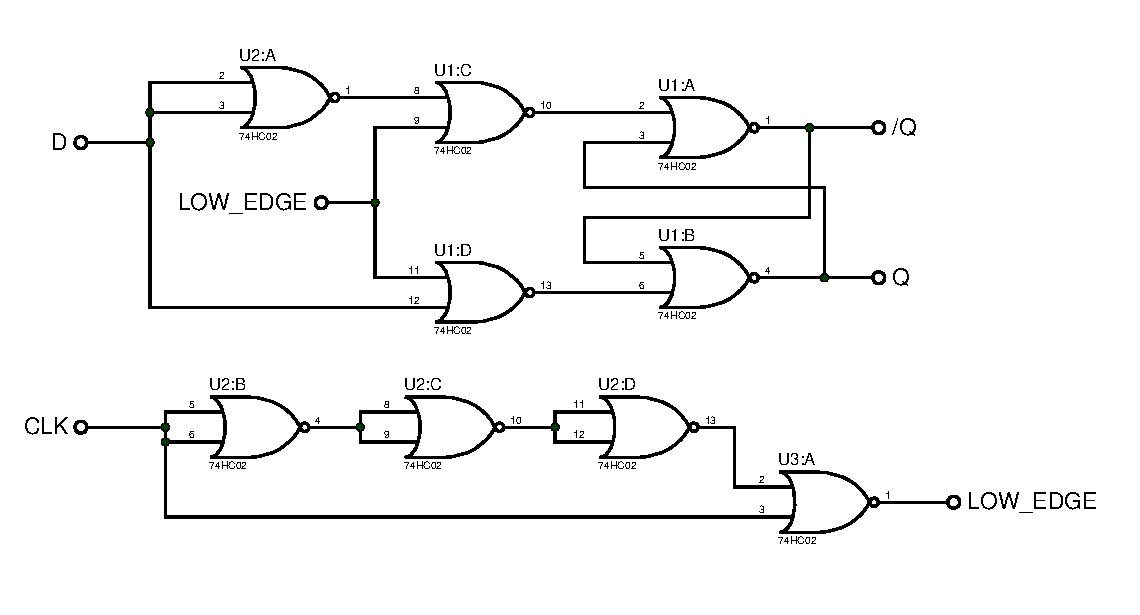
\includegraphics[width=0.9\textwidth]{dflipflop}
    \par\end{centering}
    \caption{D Flip-Flop circuit - Made in Proteus 7.8}
\end{figure}

PARAMETROS IMPORTANTES: PROPAGACION DEL D A
LA SALIDA LUEGO DEL CLK, TANTO PARA 0 COMO
PARA 1. MEDIR. COMPARAR CON UNO COMERCIAL
CUALQUIERA.

\end{document}
